\documentclass[12pt]{article}
\usepackage{amsmath}
\usepackage[margin=2.5cm]{geometry}
\usepackage[utf8]{inputenc}
\usepackage{amsfonts}
\usepackage{fancyhdr}
\usepackage{hyperref}
\usepackage{graphicx}
\usepackage{caption}
\usepackage{subcaption}
\usepackage{setspace}
\usepackage{float}
\usepackage{svg}
\setstretch{1.3} 
\usepackage{array}
\usepackage {xcolor}
%...

\usepackage{multirow} % Required for multirows




%...

%\usepackage{csc}% unknown package
\pagestyle{fancy}
\fancyhead[L]{Cubic Spline}
\fancyhead[R]{Page \thepage}
\fancypagestyle{firstpage}{%
  \lhead{}
  \rhead{}
}

\begin{document}
\begin{figure*}[!tbp]
  \begin{subfigure}[b]{0.2 \textwidth}
    
\includegraphics[width=\textwidth]{img/uni}
  \end{subfigure}
  \hfill
  \begin{subfigure}[b]{0.25\textwidth}
    
\includegraphics[width=\textwidth]{img/fani}
  \end{subfigure}
\end{figure*}
\begin{center}
\textbf{Cubic Spline} \\[1in]
Professor : Dr. Safari\\~\\
St : AmirAbbas Saberi
\\[4in]
\textbf{University of Tehran}\\
May,24,2023
\end{center}
	\thispagestyle{firstpage}
\newpage

A cubic spline is a spline constructed of piecewise third-order polynomials which pass through a set of control points. The second derivative of each polynomial is commonly set to zero at the endpoints, since this provides a boundary condition that completes the system of. equations.
\section{Cubic Spline and its error}
In general, the interpolation error with polynomials is obtained by the following method (the function must be differentiable up to degree n) \\
\begin{equation}
e_n(x) = f(x) - p(x) = \frac{f^{n+1}(\zeta)}{(n+1)!} \prod (x-x_i)
\end{equation}
SOwith some simplicity ($x_0 = a$ , $x_n = b$ , $h = \frac{b-a}{n}$)\\
\begin{equation}
|f(x) - p_n(x)| \le \frac{1}{4(n+1)}M(\frac{b-a}{n})
\end{equation}

Now the important question is how to reduce the error?

\begin{itemize}
\item Frist , Adding sampling points, which along with the possibility of derivability according to the formula we obtained, can cause problems \\for example : \\
Assume a function $f = sin(x)$ such that $a = 0$ , $b = 1.6875$ and n = 9 then 
\begin{center}
$f^{10}(x) = sin(x) \rightarrow |f^{10}(x)| \le 1 $ \\
$|sin(x) - p_n(x)| \le 1.34*10^{-9}$
\end{center}
\begin{figure}[h]
    \centering
    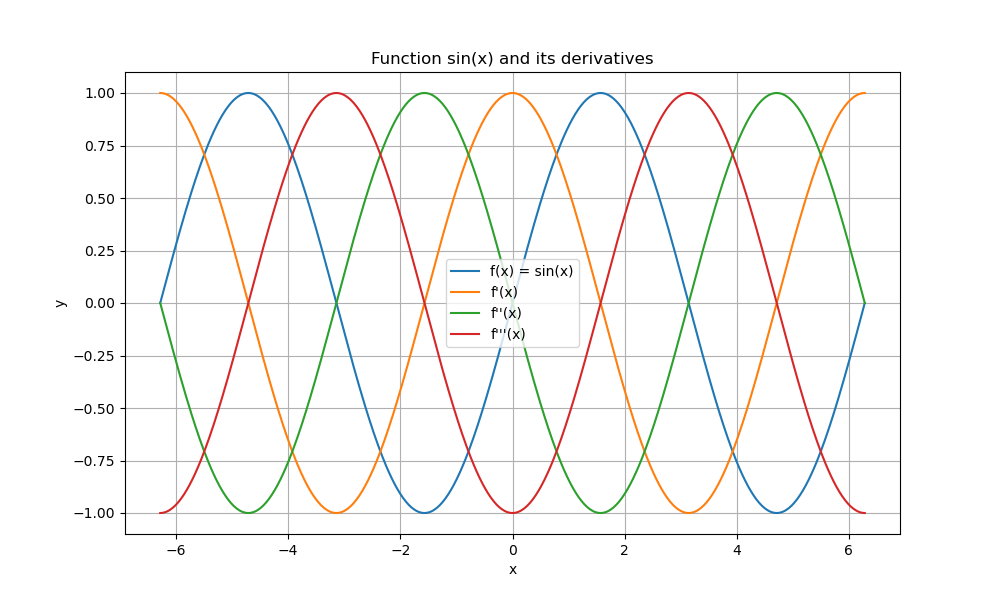
\includegraphics[width=0.5\textwidth]{img/sin}
    \caption{f = sin(x)}
    \label{fig:mesh1}
\end{figure}
\newpage
Here, adding the number of error points reduces, but let's consider another example: \\
Assume a function $f = \frac{1}{1+x^2}$
\begin{figure}[h]
    \centering
    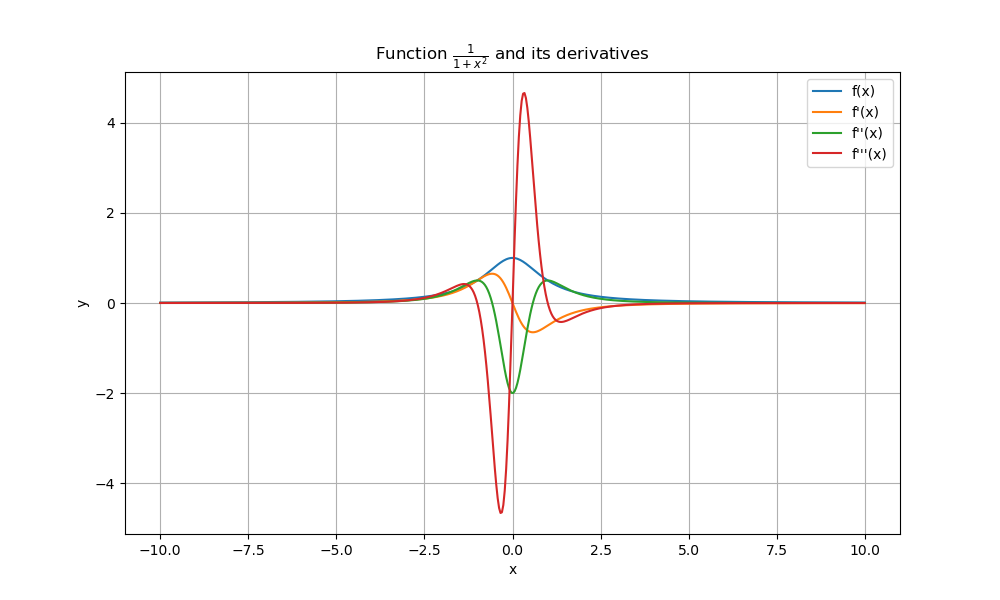
\includegraphics[width=0.8\textwidth]{img/gute}
    \caption{f = $\frac{1}{1+x^2}$ and its derivatives}
    \label{fig:mesh1}
\end{figure} \\
here is resualt of n = 20 degrees of newtoinian interpolation.
\begin{figure}[h]
    \centering
    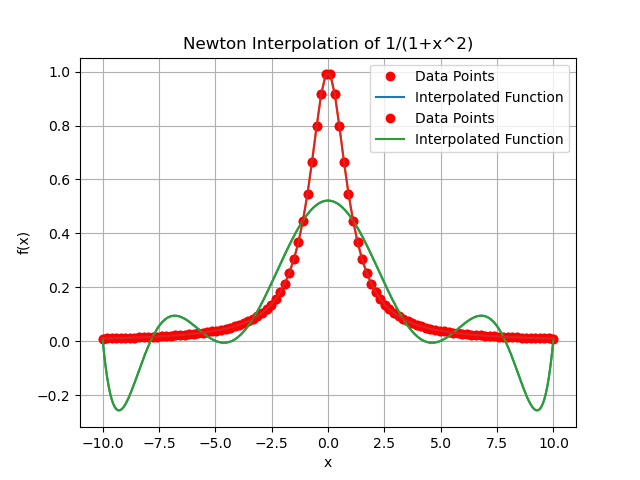
\includegraphics[width=0.5\textwidth]{img/new}
    \caption{Interpolation of f = $\frac{1}{1+x^2}$ with Newtonian method }
    \label{fig:mesh1}
\end{figure} 
\begin{equation}
P = \prod(x_i - x_j)
\end{equation}

Adding points in this function does not reduce the error, so we have to look for another way.

\item The second is to make the intervals smaller and define a separate polynomial for each small interval.

\begin{equation}
  S_{m,n}=\begin{cases}
    p_{1}(x) = a_0^1 + a_1^1 x + a_2^1 x^2 + ... + a_m^1 x^m\\
    p_{2}(x) = a_0^2 + a_1^2 x + a_2^2 x^2 + ... + a_m^2 x^m\\
    .\\
    .\\
    .\\
    p_{n}(x) = a_0^n + a_1^n x + a_2^n x^2 + ... + a_m^n x^m
  \end{cases}
\end{equation}
In this project, we work with a cubic spline that: \\
\begin{equation}
  S_{3,n}=\begin{cases}
    p_{1}(x) = a^1_{3}x^3 + a^1_{2}x^2 + a_{1}^1x + a_0^1\\
    p_{2}(x) = a^2_{3}x^3 + a^2_{2}x^2 + a_{1}^2x + a_0^2\\
    .\\
    .\\
    .\\
    p_{n}(x) = a^n_{3}x^3 + a^n_{2}x^2 + a_{1}^nx + a_0^n
  \end{cases}
\end{equation}

\begin{equation}
  4n-2 = \begin{cases}
   1) p'_i(x) = p'_{i+1}(x) , [i = 1,...,n-1]\\
   2) \ddot{p}_i(x) = \ddot{p}_{i+1}(x) , [i = 1,...,n-1]\\
   3) p'_i(x_i) = f_{i-1}) , [i = 1,...,n]\\
   4) p'_i(x) = f_{i} , [i = 1,...,n]
  \end{cases}
\end{equation}
We have two conditions to obtain low coefficients :\\
\begin{itemize}
\item Natural \begin{equation}
 \begin{cases}
   1) s'_{3,n}(a) = s'_{3,n}(b) = 0\\
   2) \ddot{s}_{3,n}(a) = \ddot{s}_{3,n}(b) = 0
  \end{cases}
\end{equation}
\item Periodic 
\begin{equation}
s^{k}_{3,n}(a) = s^{k}_{3,n}(b) \leftarrow k = [0,1,2]
\end{equation}
\item Conditional
\begin{equation}
\begin{cases}
   1) s'_{3,n}(a) = f'_0\\
   2) s'_{3,n}(b) = f'_n
  \end{cases}
\end{equation}
\end{itemize} 

Theorem: Suppose $\ddot{f}$ is continuous in a and b, and if S is the cubic interpolator function of f in the nodes ti and $0 \le i < n $ then: \\ 
\centerline{
\(\int_{a}^{b} [ \ddot{s}(x) ]^2 \,dx\) $\le$ \(\int_{a}^{b} [ \ddot{f}(x) ]^2 \,dx\)}\\
A conclusion can be drawn from the above case : \\
\begin{equation}
s(x) = \sum\limits_{i=0}^m a_i x + \sum\limits_{i=0}^m b_i (x-x_i) ^{2m+1}
\end{equation}
and 
\begin{equation}
e_n(x) = \frac{(b-4)^4}{24n^4} max|f^{(4)}(x)|
\end{equation} \\
The error is reduced by a factor of $\frac{1}{n^4}$ \\
\begin{equation}
s(x) = Ab
\end{equation}
\begin{equation}
A = \begin{bmatrix}
1 & x_1 & 0 & 0 & 0 &. & . & . & 0 \\
1 & x_2 & (x_2 - x_1)^3 & 0 & 0 & . & . & . & 0 \\
1 & x_3 & (x_3 - x_1)^3 & (x_3 - x_2)^3 & 0 & . & . & . & 0 \\
. & . & . & . & . & . & . & . & . \\
. & . & . & . & . & . & . & . & . \\
. & . & . & . & . & . & . & . & . \\
1 & x_n & (x_n - x_1)^3 & (x_n - x_2)^3 & 0 & . & . & . & (x_n - x_{n-1})^3 \\
0 & 0 & 1 & 1 & . & . & . & 1 & 1 \\
0 & 0 & x_1 & x_2 & . & . & . & . & x_n


\end{bmatrix}
\end{equation}
\begin{equation}
b = A^{-1}s
\end{equation}
\newpage
\section{Example of Natural Cubic Spline and Linear Spline}
\subsection{f = $\frac{1}{1+x^2}$}
Consider the f function as the $\frac{1}{1+x^2}$ function\\
\begin{figure}[h]
    \centering
    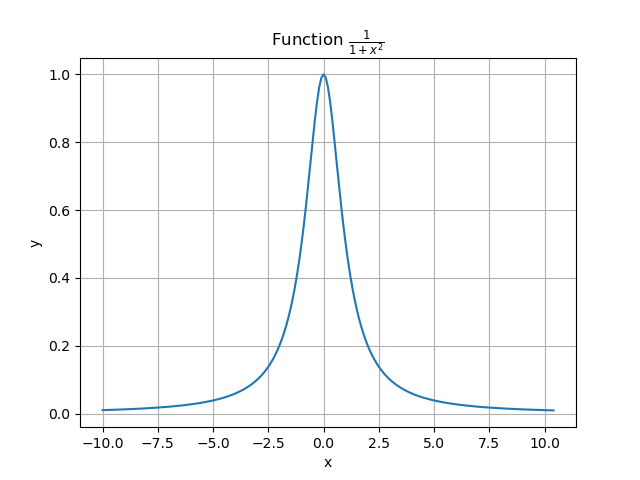
\includegraphics[width=0.5\textwidth]{img/gute1}
    \caption{f = $\frac{1}{1+x^2}$}
    \label{fig:mesh1}
\end{figure}
We consider the sampling step length of the function to be 0.25 and apply a cubic spline to the resulting sample \\
\begin{figure}[h]
    \centering
    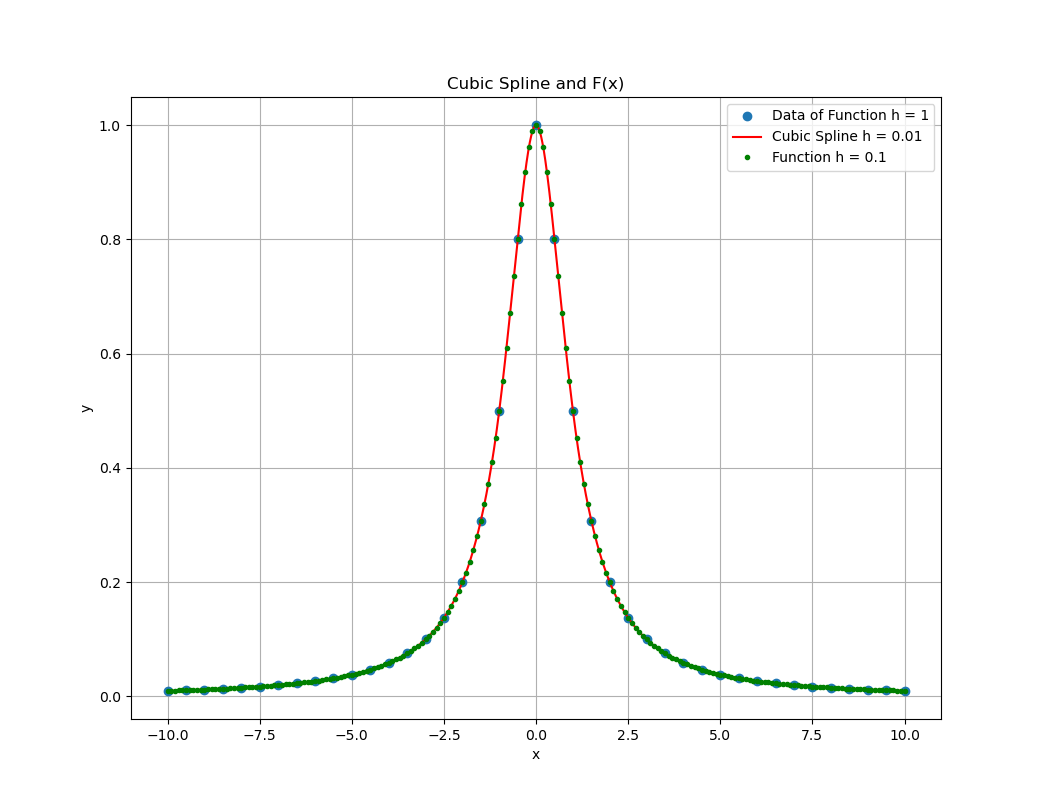
\includegraphics[width=0.6\textwidth]{img/gute2}
    \caption{Spline of f , sample (h = 1) with $h_s = 0.01$ }
    \label{fig:mesh1}
\end{figure}\\

\begin{figure}[h]
    \centering
    \includegraphics[width=0.6\textwidth]{img/Spline_Linear}
    \caption{Spline of f , sample (h = 1) with $h_s = 0.01$}
    \label{fig:mesh1}
\end{figure}

\newpage

error with real functions (step length of the spline to be 0.01) : \\
\begin{table}[h!]
  \begin{center}
    \caption{Table of Spline Error.}
    \label{tab:table1}
    \begin{tabular}{c|c}
      \multicolumn{2}{c}{e = $f - \hat{s}$}\\
      \hline
      \multirow{1}{*}{Cubic} & \multirow{1}{*}{Linear} \\
      \hline
      \multirow{2}{*}{0.00155} & \multirow{2}{*}{0.0255}
      
    \end{tabular}
  \end{center}
\end{table}
\newpage
\subsection{f = $11 (cos(0.5x))^2 + x^4 + 7 sin(2x)$}
Consider the f function as the $\frac{1}{1+x^2}$ function\\
\begin{figure}[h]
    \centering
    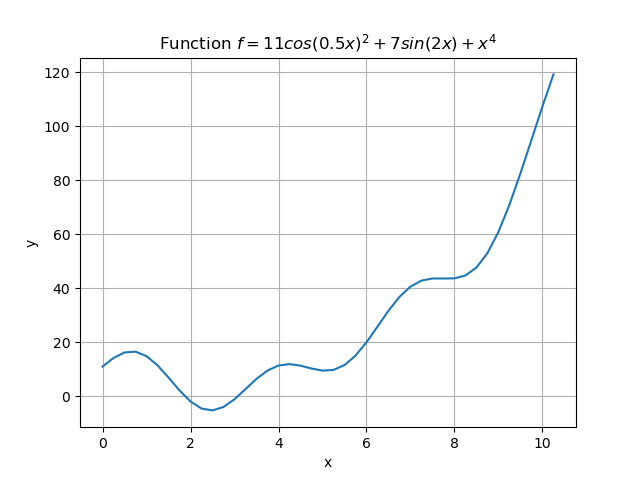
\includegraphics[width=0.5\textwidth]{img/f}
    \caption{f = $11 (cos(0.5x))^2 + x^4 + 7 sin(2x)$}
    \label{fig:mesh1}
\end{figure}
We consider the sampling step length of the function to be 0.25 and apply a cubic spline to the resulting sample \\
\begin{figure}[h]
    \centering
    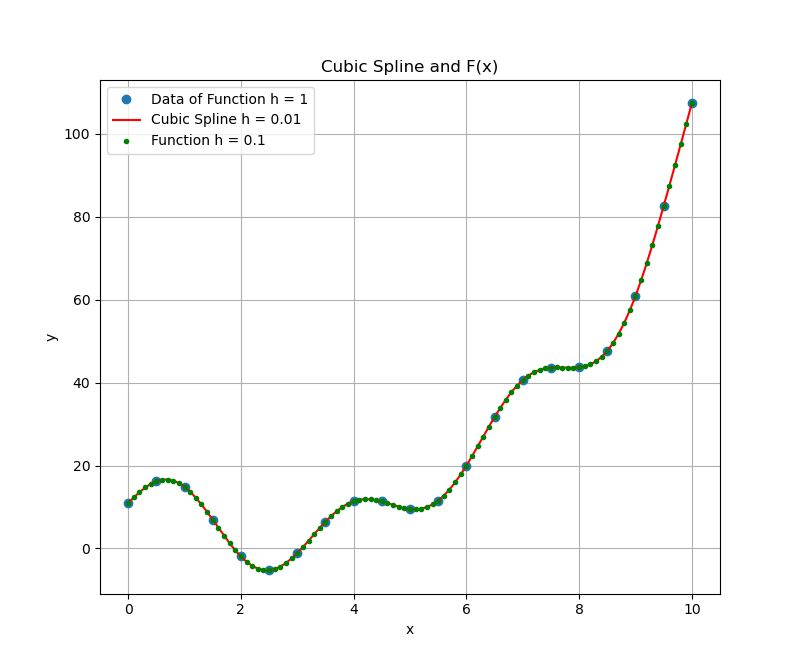
\includegraphics[width=0.6\textwidth]{img/f1}
    \caption{Spline of f , sample (h = 1) with $h_s = 0.01$}
    \label{fig:mesh1}
    
\end{figure}\\

\begin{figure}[h]
    \centering
    \includegraphics[width=0.6\textwidth]{img/Spline_Linear2}
    \caption{Spline of f , sample (h = 1) with $h_s = 0.01$}
    \label{fig:mesh1}
\end{figure}

\newpage

error with real functions (step length of the spline to be 0.01) : \\
\begin{table}[h!]
  \begin{center}
    \caption{Table of Spline Error.}
    \label{tab:table1}
    \begin{tabular}{c|c}
      \multicolumn{2}{c}{e = $f - \hat{s}$}\\
      \hline
      \multirow{1}{*}{Cubic} & \multirow{1}{*}{Linear} \\
      \hline
      \multirow{2}{*}{0.0726} & \multirow{2}{*}{0.1327}
      
    \end{tabular}
  \end{center}
\end{table}

\end{itemize}


\end{document}